%%%%%%%%%%%%%%%%%%%%%%%%%%%%%%%%%%%%%%%%%%%%%%%%%%%%%%%%%%%%%%%
%
% Welcome to writeLaTeX --- just edit your LaTeX on the left,
% and we'll compile it for you on the right. If you give
% someone the link to this page, they can edit at the same
% time. See the help menu above for more info. Enjoy!
%
%%%%%%%%%%%%%%%%%%%%%%%%%%%%%%%%%%%%%%%%%%%%%%%%%%%%%%%%%%%%%%%

% --------------------------------------------------------------
% This is all preamble stuff that you don't have to worry about.
% Head down to where it says "Start here"
% --------------------------------------------------------------
 
\documentclass[12pt]{article}
 
\usepackage[margin=1in]{geometry}
\usepackage{amsmath,amsthm,amssymb}

\usepackage{listings}
\usepackage{xcolor}
\usepackage{graphicx}
\graphicspath{{./images/}}

\usepackage{tikz}
\usetikzlibrary{shapes,positioning}

\tikzset{ell/.style={circle,draw,minimum height=0.5cm,minimum width=0.5cm,inner sep=0.2cm}}
\tikzset{rec/.style={rectangle,draw,minimum height=0.5cm,minimum width=0.5cm,inner sep=0.2cm}}
%New colors defined below
\definecolor{codegreen}{rgb}{0,0.6,0}
\definecolor{codegray}{rgb}{0.5,0.5,0.5}
\definecolor{codepurple}{rgb}{0.58,0,0.82}
\definecolor{backcolour}{rgb}{0.95,0.95,0.92}

%Code listing style named "mystyle"
\lstdefinestyle{mystyle}{
  backgroundcolor=\color{backcolour}, commentstyle=\color{codegreen},
  keywordstyle=\color{magenta},
  numberstyle=\tiny\color{codegray},
  stringstyle=\color{codepurple},
  basicstyle=\ttfamily\footnotesize,
  breakatwhitespace=false,         
  breaklines=true,                 
  captionpos=b,                    
  keepspaces=true,                 
  numbers=left,                    
  numbersep=5pt,                  
  showspaces=false,                
  showstringspaces=false,
  showtabs=false,                  
  tabsize=2
}

%"mystyle" code listing set
\lstset{style=mystyle}

 
\newcommand{\N}{\mathbb{N}}
\newcommand{\Z}{\mathbb{Z}}
 
\newenvironment{theorem}[2][Theorem]{\begin{trivlist}
\item[\hskip \labelsep {\bfseries #1}\hskip \labelsep {\bfseries #2.}]}{\end{trivlist}}
\newenvironment{lemma}[2][Lemma]{\begin{trivlist}
\item[\hskip \labelsep {\bfseries #1}\hskip \labelsep {\bfseries #2.}]}{\end{trivlist}}
\newenvironment{exercise}[2][Exercise]{\begin{trivlist}
\item[\hskip \labelsep {\bfseries #1}\hskip \labelsep {\bfseries #2.}]}{\end{trivlist}}
\newenvironment{problem}[2][Problem]{\begin{trivlist}
\item[\hskip \labelsep {\bfseries #1}\hskip \labelsep {\bfseries #2.}]}{\end{trivlist}}
\newenvironment{question}[2][Question]{\begin{trivlist}
\item[\hskip \labelsep {\bfseries #1}\hskip \labelsep {\bfseries #2.}]}{\end{trivlist}}
\newenvironment{corollary}[2][Corollary]{\begin{trivlist}
\item[\hskip \labelsep {\bfseries #1}\hskip \labelsep {\bfseries #2.}]}{\end{trivlist}}

\newenvironment{solution}{\begin{proof}[Solution]}{\end{proof}}
 
\begin{document}
 
% --------------------------------------------------------------
%                         Start here
% --------------------------------------------------------------
 
\title{Test 2}%replace X with the appropriate number
\author{Mengxiang Jiang\\ %replace with your name
CSEN 5322 Operating Systems} %if necessary, replace with your course title
 
\maketitle
 
\begin{problem}{1} %You can use theorem, exercise, problem, or question here.  Modify x.yz to be whatever number you are proving
  Consider the following set of resource allocations and requests. Process
  1 holds resources A, B, and C and is waiting for resource D. Process 2 holds resource E and
  is waiting for resource C. Process 3 holds resource D and is waiting for resource E.\\\\
  a) Draw a Resource Allocation Graph (RAG) for the situation given above. Use circular
  nodes for processes and square nodes for resources.\\\\
  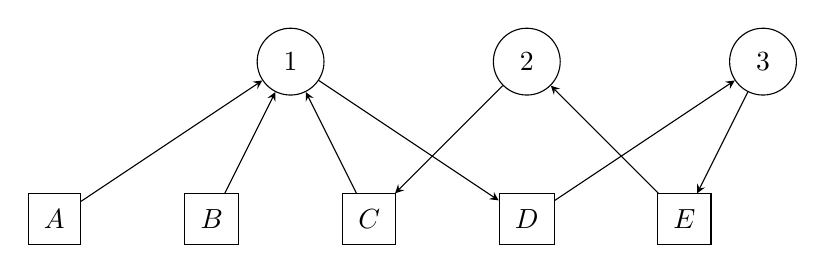
\begin{tikzpicture}[>=stealth]
    \node[ell] (p1)at (3,0) {$1$};
    \node[ell] (p2)at (6,0) {$2$};
    \node[ell] (p3)at (9,0) {$3$};
    \node[rec] (a)at (0,-2) {$A$};
    \node[rec] (b)at (2,-2) {$B$};
    \node[rec] (c)at (4,-2) {$C$};
    \node[rec] (d)at (6,-2) {$D$};
    \node[rec] (e)at (8,-2) {$E$};

    \draw [->] (a) to []node[]{} (p1);
    \draw [->] (b) to []node[]{} (p1);
    \draw [->] (c) to []node[]{} (p1);
    \draw [->] (p1) to []node[]{} (d);
    \draw [->] (e) to []node[]{} (p2);
    \draw [->] (p2) to []node[]{} (c);
    \draw [->] (d) to []node[]{} (p3);
    \draw [->] (p3) to []node[]{} (e);
\end{tikzpicture}
\\(b) Is there a deadlock present in the system? If so, which processes and resources are
involved? If not, give an ordering that the processes can run in to complete execution.\\
Yes, there's a deadlock since there's a cycle where 1 needs D, but D is held by 3, 3 needs E, but E is held by 2, and 2 needs C, but C is held by 1.
\end{problem}

\begin{problem}{2}
  Suppose that a machine has 38-bit virtual addresses and 32-bit physical addresses\\
  (a) What is the main advantage of a multilevel page table over a single-level one?\\
  Multilevel allows keeping all page table entries in memory rather than some in disk (which is much slower).\\\\
  (b) With a two-level page table, 16-KB pages, and 4-byte entries, how many bits should be allocated
  for the top-level page table field and how many for the next level page table field? Explain.\\
  12 bits for each of the three page fields. Offset requires 14 bits to address 16KB ($2^4*2^{10} = 2^{14}$). Each entry being 4 bytes so one page holds $2^{12}$ page table entries, so 12 bits for each will address all $2^{12}*2^{14}*2^{12}=2^{38}$ bytes.
\end{problem}
\pagebreak
\begin{problem}{3}
  A computer has four-page frames. The time of loading, time of last access,
and the R and M bits for each page are as shown below (the times are in clock ticks):
\begin{tabular}{|c c c c c|} 
  \hline
  Page & Loaded & Last ref. & R & M\\
  \hline
  0 & 126 & 280 & 1 & 0\\
  1 & 230 & 265 & 0 & 1\\
  2 & 140 & 270 & 0 & 0\\
  3 & 110 & 285 & 1 & 1\\
  \hline
 \end{tabular}
 \\(a) Which page will NRU replace?\\
 Page 2 since the referenced and modified bits are 0.\\\\
 (b) Which page will LRU replace?\\
 Page 1 since the last referenced was 265, which is the oldest referenced.\\\\
 (c) Which page will FIFO replace?\\
 Page 3 since it was loaded at 110, which is the oldest load.\\\\
 (d) Which page will second chance replace?\\
 Page 1 since the referenced bit is 0 and it is the oldest referenced so it will be in front of 2 in the queue.
\end{problem}

\begin{problem}{4}
  In the WSClock algorithm of Fig, the hand points to a page with R = 0. If $\tau$ = 400, will
this page be removed? What about if $\tau$ = 1000?\\
\begin{figure}[ht]
  \centering
  \includegraphics[scale=0.7]{clock}
\end{figure}
\\If $\tau = 400 \rightarrow 2204-1213 = 991 > 400$, so the page is removed.\\
\\If $\tau = 1000 \rightarrow 2204-1213 = 991 < 1000$, so the page is kept.\\
\end{problem}
\pagebreak
\begin{problem}{5}
  A system has two processes and three identical resources. Each process needs a
maximum of two resources. Is deadlock possible? Explain your answer.\\
No, at least one of the processes will obtain the two resources it needs to run to completion, allowing the second to then acquire the free resources to also run to completion.
\end{problem}

\begin{problem}{6}
  (a) Show the derivation of the optimum page size equation, $o = \sqrt{2pt}$,
where the average process size is $p$ bytes (total virtual space), each page table entry required
$t$ bytes, and the page size is $o$ bytes.\\
Page table entries will be $\frac{p}{o}t$ bytes.\\
Average of $\frac{o}{2}$ bytes wasted on last page.\\
Total overhead $f(p)= (\frac{p}{o}t) + \frac{o}{2}$\\
$f(p)' = -\frac{pt}{o^2} + \frac{1}{2} \rightarrow -\frac{pt}{o^2} = -\frac{1}{2} \rightarrow o^2 = 2pt \rightarrow o = \sqrt{2pt}$\\\\
(b) For, p = 4MB and t = 8 bytes per page table entry, what is the optimum page size?\\
$o = \sqrt{2pt} = \sqrt{2*4*1024*1024*8} = 8192$ bytes or 8 KB.
\end{problem}

\begin{problem}{7}
  Suppose that a machine has 48-bit virtual addresses and 32-bit physical
addresses. If pages are 4 KB, how many entries are in the page table if it has only a singlelevel? Explain.\\
$\frac{2^{48}}{2^{12}} = 2^{36} \approx 69$ Billion entries.
\end{problem}
% --------------------------------------------------------------
%     You don't have to mess with anything below this line.
% --------------------------------------------------------------
 
\end{document}